\item In the arrangement shown in Fig. 1.49 the mass of body 1 is $\eta=4.0$ times as great as that of body 2. The height $h=20 \text{ cm}$. The masses of the pulleys and the threads, as well as the friction, are negligible. At a certain moment body 2 is released and the arrangement set in motion. What is the maximum height that body 2 will go up to?
    \begin{center}
        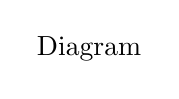
\begin{tikzpicture}
            \node at (0, 0) {Diagram};
        \end{tikzpicture}
    \end{center}
\begin{solution}
    \begin{center}
        \begin{tikzpicture}
            \pic at (0, 0) {frame=3cm};
        \end{tikzpicture}
    \end{center}
    
    \begin{align*}
        \intertext{Using Newton’s second law in projection form along $x$-axis for the body 1 and along negative $x$-axis for the body 2, respectively, we get}
        m_1g - T_1 &= m_1w_1 \tag{1}\\
        T_2 - m_2g &= m_2w_2 \tag{2}\\
        \intertext{For the pulley lowering in downward direction from along $x$-axis, Newton’s law gives}
        T_1 - 2T_2 &= 0 \quad \text{(as pulley is massless)} \tag{3}\\
        \intertext{or}
        T_1 &= 2T_2\\
        \intertext{As the length of the thread is constant, so}
        w_2 &= 2w_1 \tag{4}\\
        \intertext{The simultaneous solution of above equations yields}
        w_2 &= \dfrac{2(m_1 - 2m_2)g}{4m_2 + m_1} = \dfrac{2(\eta - 2)}{\eta + 4}g \quad \bigg(\text{as } \dfrac{m_1}{m_2} = \eta \bigg) \tag{5}\\
        \intertext{Obviously during the time interval in which the body $1$ comes to the horizontal floor covering the distance $b$, the body $2$ moves upward the distance $2b$. At the moment when the body $2$ is at the height $2b$ from the floor its velocity is given by the expression}
        v_2^2 &= 2w_2 (2b) = 2 \left[ \dfrac{2(\eta - 2)}{\eta + 4} g \right] 2b = \dfrac{8b(\eta - 2)g}{\eta + 4}\\
        \intertext{After the body $m_1$ touches the floor, the thread becomes slack or the tension in the thread zero, thus as a result body 2 is only under gravity for its subsequent motion.}
        \intertext{Owing to the velocity $v_2$ at that moment or at the height $2b$ from the floor, the body 2 further goes up under gravity by the distance,}
        h' &= \dfrac{v_2^2}{2g} = \dfrac{4b(\eta - 2)}{\eta + 4}\\
        \intertext{Thus the sought maximum height attained by body 2 is}
        H &= 2b + h' = 2b + \dfrac{4b(\eta - 2)}{\eta + 4}\\
        &= \dfrac{6\eta b}{\eta + 4} = 0.6\, \text{m} \quad \text{(on substituting values)}
    \end{align*}
\end{solution}
